\documentclass[12pt]{article}
 
% ---- Packages ----
\usepackage{amsmath,amssymb}
\usepackage[T1]{fontenc}
\usepackage[utf8]{inputenc}
\usepackage{lmodern}
\usepackage[margin=1in]{geometry}
\usepackage{setspace}
\usepackage{graphicx}
\usepackage{float}
\usepackage{booktabs}
\usepackage{natbib}
\usepackage{hyperref}
\usepackage{titling}
\usepackage{tabularray}
\UseTblrLibrary{booktabs}
 
% ---- Double spacing ----
\doublespacing
 
% ---- Float placement: tables and figures at end ----
\floatplacement{figure}{p}
\floatplacement{table}{p}
 
\title{Immigration Enforcement and Labor Market Effects\\
       in Immigrant-Intensive Industries}
\author{Bee Nguyen\\
        \small Department of Economics, University of Oklahoma}
\date{April 2026}


% ---- Bibliography style ----
\bibliographystyle{aer}
 
\begin{document}
 
\begin{titlepage}
    \centering
    \vspace*{3cm}
    {\LARGE\bfseries Immigration Enforcement and Labor Market Effects\\[0.3cm]
    in Immigrant-Intensive Industries\par}
    \vspace{1.5cm}
    {\large Bee Nguyen\par}
    {\normalsize Department of Economics, University of Oklahoma\par}
    \vspace{1cm}
    {\large April 2026\par}
    \vspace{2cm}

\end{titlepage}
\begin{abstract}
This paper examines the effect of the 2017 immigration enforcement surge on 
employment in immigrant-intensive industries across U.S. metropolitan statistical 
areas. Using a difference-in-differences event study design, I compare employment 
trajectories in states with above-median pre-treatment immigrant labor concentration 
to those with below-median concentration in agriculture, construction, food 
manufacturing, and food services. Treatment status is constructed from CPS ASEC 
microdata (2014--2020), and outcomes are measured using QCEW county-level 
employment data aggregated to the MSA level. Contrary to expectations, high-immigrant 
states experienced statistically significant employment growth in target industries 
relative to low-immigrant states following 2017, with estimates of approximately 
5 percent by 2018. Robustness checks substituting immigrant employment as the 
outcome variable produce uniformly insignificant estimates, suggesting the main 
results reflect broader macroeconomic trends rather than a direct enforcement 
effect. Results are robust to the exclusion of sanctuary states. These findings 
highlight the difficulty of isolating immigration enforcement effects from 
contemporaneous economic expansion and point to the need for more granular 
enforcement measures in future work.
\end{abstract}

\newpage
 

\section{Introduction}

 
The United States experienced a significant shift in immigration enforcement following the 2017 presidential transition, driven by executive orders expanding interior enforcement and broadening deportation priorities. These policies created substantial labor supply shocks in industries historically dependent on immigrant workers, including food services, construction, and food manufacturing. Analyzing the effects of these enforcement changes allows us to evaluate the economic costs associated with restrictive immigration policy and provides insight into the potential impacts of current enforcement efforts under the second Trump administration.

This paper examines whether states with higher pre-existing immigrant labor concentration in target industries experienced greater employment declines following the 2017 enforcement surge relative to states with lower immigrant labor dependence. Using microdata from the Current Population Survey Annual Social and Economic Supplement (CPS ASEC) accessed via IPUMS for 2014–2020 cross walked with QCEW Data, we employ a difference-in-differences strategy to estimate the differential employment effects of the enforcement shock. States are classified as high-exposure based on their pre-treatment immigrant labor share in agriculture, construction, food manufacturing, and food services.
 
\section{Literature Review}

The discussion about immigration in regard to policy enforcement has always been a debate during every single presidential election. As we move into a new age of American politics, it is important now than ever to evaluate previous administrative actions on immigration policy to help gauge the importance of current enforcement. It is undeniable that immigrants bring immense value to many different industries in the United States. In fact, \citet{borjas2019} acknowledges in his working paper that immigration broadly affects economic growth through its interaction with capital accumulation and labor market competition, though he notes the distributional effects are uneven especially with native workers in directly competing roles potentially facing wage pressure while the broader economy benefits. The direction I want to take with this paper is to address the importance of workers in industries that might not necessarily be classified as ``high-skilled'', such as fast-food or construction. I must preface that it doesn't mean that these industries lack skilled labor, but rather when compared to industries that require professional degrees, one could argue the accessibility varies greatly. This matters greatly as many immigrants who are vulnerable to enforcement policies fall under the umbrella of these target industries.

While this paper utilizes data on formal reports of employment through employers of surveys, it is important to note the impacts of undocumented immigrants participating in these target industries. Throughout the presidential debate of 2016, the topic of unauthorized workers was a main front into incorporating effective immigration policies. Philip Martin notes in his paper that the sheer degree of Trump's plans to restrict immigration through extensive means could be ``disruptive to American agriculture'' \citep[p.~1]{martin2017}. What this paper analyzes is to what degree do these policies affect immigrant heavy industries such as agriculture. The mission to bring back jobs for American citizens through extensive citizenship application requirements and lengthened citizenship processes potentially poses a harm into industries that rely on immigrant labor. Additionally, enforcing these policies require extensive expenditures of tax payer dollars, which ironically the same immigrants pay towards. Humanitarian programs were actually being cut off from federal funding as a result of these enforcement initiatives \citep[p.~6]{pierce2018}. Analysis of the effects of the removal of these programs isn't necessarily captured in my paper, but the implications of changes in total employment could run into government funded programs like SNAP and Social Security.

Building on this body of work, the theoretical foundation for understanding why enforcement driven reductions in immigrant labor do not necessarily translate into job gains for native workers has been well established. Research about this reveals that because immigrant and native workers tend to fill complementary roles rather than directly competing ones, removing immigrant labor can actually hurt overall job creation in affected industries \citep{chassamboulli2015}. This is particularly relevant to the target industries this paper covers. When thinking about this empirically, immigration enforcement has been found to significantly reduce immigrant employment with spillover effects onto native workers in related roles \citep{east2023}. What my goal for this paper is to build on these findings by applying a difference-in-differences strategy at the MSA level, using pre-existing immigrant labor concentration as a way to measure which states were more exposed to the 2017 enforcement surge and evaluating how that exposure translated into changes in total employment across our target industries.

 
\section{Data}
 
This paper uses two primary data sources linked through a geographic
crosswalk.
 
\textbf{CPS ASEC.} The primary source for constructing the pre-treatment variables is the CPS ASEC microdata accessed via IPUMS, covering the years 2014-2020. The CPS ASEC is a nationally representative survey of U.S. households that combines data across the US Census Bureau and the Bureau of Labor Statistics. The sample is restricted to individuals
aged 16--64 years who are ASEC respondents with non-missing employment status. The immigrant status is defined as foreign-born (NATIVITY $\neq$ 1). Target industries are identified using CPS industry codes corresponding to agriculture, construction, food manufacturing, and food services. I used the CPS data to specifically construct the pre-treatment immigrant labor share by state and used those numbers to determine which states classified as high immigrant or low immigrant in our target industries. It is important to note that the IPUMS industry classification is based on the 2017 Census Classification Scheme, which lists out the numerous industries that compose the labor force. This code system is not the same as QCEW. 
 
\textbf{QCEW.} The primary outcome data comes from the QCEW, which I accessed through the BLS public API. The QCEW is an employer-reported dataset that provides annual average employment counts and average annual pay at the county level by NAICS industry code. I specifically pulled data for the four target industries (agriculture, NAICS 11; construction, NAICS 23; food manufacturing, NAICS 311; and food services, NAICS 722) for all counties within metropolitan statistical areas from 2014 to 2020. Since the QCEW reports at the county level but my analysis is at the MSA level, I used a Census Bureau reference file that maps each county to its corresponding metro area to conjure the county employment counts up to the MSA level. This gives me total employment in target industries for each MSA in each year, which serves as the main outcome variable in the difference-in-differences regression.
 
\textbf{Crosswalk.} Since the QCEW and CPS data are organized at different geographic levels, I needed a way to connect them. I did this by using a Census Bureau reference file that links each county to its metro area, which allowed me to match MSA-level employment outcomes from the QCEW to the state-level immigrant share classifier from the CPS. One limitation worth noting is that some metro areas span across two states, like Kansas City spanning Missouri and Kansas. In those cases I just kept the first state match, which means some border MSAs may be assigned the wrong state's immigrant share.
 
\textbf{Summary Statistics.} Table 1 presents summary statistics for
the analysis sample.

\section{Empirical Methods}

This paper uses a difference-in-differences design to estimate the causal effect of the 2017 immigration enforcement surge on employment in immigrant-intensive industries. The main specification is estimated as an event study:

\begin{equation}
Y_{mt} = \alpha + \sum_{\tau \neq 2016} \beta_\tau (HighImmigrant_s \times \mathbf{1}[\tau = t]) + \gamma_m + \delta_t + \varepsilon_{mt}
\end{equation}

where $Y_{mt}$ is log total employment in target industries for MSA $m$ in year $t$. $HighImmigrant_s$ equals one if the state containing MSA $m$ had an above-median immigrant labor share in target industries during 2014--2016, constructed from CPS ASEC microdata. Rather than producing a single average post-treatment estimate, this specification produces a separate coefficient $\beta_t$ for each year relative to 2016, allowing me to trace how effects evolved over time. MSA fixed effects $\gamma_m$ absorb time-invariant differences across metro areas, and year fixed effects $\delta_t$ absorb economy-wide shocks common to all MSAs in a given year. Standard errors are clustered at the state level since treatment is assigned at the state level. Additionally, States below the median pre-treatment immigrant labor share serve as the control group, as they were less exposed to the enforcement shock and provide the counterfactual 
employment trend for high-immigrant states. 

The identifying assumption is parallel trends: in the absence of the 2017 enforcement surge, employment in target industries would have evolved similarly across high and low immigrant states. This assumption is assessed by examining the pre-period coefficients for 2014 and 2015, which should be statistically indistinguishable from zero if the assumption holds.

To construct $HighImmigrant$, we utilize CPS data by aggregating all observations classified with a nativity value not equal to 1 and divide that sum by the total observations per state, including Washington D.C. This value is our immigration concentration, which details the portion of observations classified as an immigrant in our sample. Since we have an immigration concentration value for each state, we can set a threshold to classify if each state has a high immigrant share or low immigrant share based on their concentration value. Using the median is preferable to the mean as it is robust to outliers which are the states with extremely high immigrant concentrations like California and New York would skew a mean-based threshold upward, potentially misclassifying states. The median guarantees an equal split between our treatment and control groups regardless of the distribution of immigrant shares across states.

As a robustness check, we substitute our outcome variable with immigrant employment. This allows us to assess whether changes in total employment are specifically impacting immigrants or whether changes in total employment are driven by macroeconomic factors that confound our model. Calculating immigrant employment requires us to multiply the immigrant concentration value by the total employment found in our QCEW dataset for every MSA based on their associated STATEFIP code. It is important to note that when constructing the CPS/QCEW panel, we assign certain cross-state MSAs to a single state in which they are mostly contained. This could affect our identification strategy as we cluster results at the state level, subjecting border MSAs to the effects of states they do not entirely reside in.

An additional robustness check we implement is to exclude states with sanctuary policies. Research has shown that sanctuary policies meaningfully reduce deportations of non-criminal immigrants, suggesting that high-immigrant states with sanctuary designations may have faced systematically lower enforcement intensity than our treatment variable implies \citep{hausman2020}. Removing these states allows us to isolate changes in total employment to states that would be most vulnerable to the enforcement shock.

The treatment timing of 2017 is not chosen at random as it pertains to the inauguration of the first Trump Administration. However, a caveat worth noting is that policy implementation did not occur until late 2017 or early 2018 for many enforcement directives. This affects the interpretation of our 2017 coefficient specifically, as the full enforcement effect may not yet be captured in that year, which is an additional assumption embedded in our use of 2016 as the reference year.

 
\section{Findings}

The main event study results are reported in Table 2 and visualized in Figure 1.

Contrary to our expectations, the DID regression model reveals that our target industries (agriculture, food manufacturing, food service, and construction) saw increases in total employment relative to our reference year (2016). Firstly, our expectations of our timing assumption for 2017 makes sense as estimates across all models and robustness checks are small and statistically insignificant. This pairs with the fact that enforcement policy was not implemented until either late that year or early the following year. From our main model, we observe that our estimates from 2018 to 2020 are statistically significant. In 2018, high-immigrant states saw total employment in target industries grow by approximately 5.1 percent more than low-immigrant states, relative to their shared 2016 baseline. In 2019 and 2020, we observe statistically significant estimates of 4.69 and 4.73 percent respectively. This is surprising because we expect immigration enforcement protocols to prohibit or stagnate growth in these industries as a result.

One thing to note about our estimates across all models is the pre-trends assumption. For our main model, we observe that the estimates for 2014 and 2015 were small and statistically insignificant at -0.011 and -0.004 respectively. In our first robustness check model that uses logged immigrant employment as the outcome variable, our estimates for 2014 and 2015 were 0.069 and 0.028 respectively. In our second robustness check with sanctuary states removed, our estimates for 2014 and 2015 were -0.010 and -0.008 respectively. Both robustness checks displayed statistically insignificant estimates that were marginal, which supports our parallel trends assumption necessary for performing a difference-in-differences regression.

Pivoting to our first robustness check, we can observe that all our estimates are statistically insignificant. This is important in revealing how changing the specificity of our model alters the results of our regression. What this entails for our interpretation is that there is no statistically significant impact of the 2017 policy surge on immigrant labor numbers between high and low immigrant concentration states. It is important to note that we utilized a projection method that estimates the number of employed immigrants per MSA relative to the state's immigrant concentration. While this provides us with a simple projection of the potential number of workers who classify as immigrant in our target industries, it still remains a limitation in how we use immigrant employment as an identification feature in our robustness check. Taking that into account, further research and data gathering would be necessary to determine the impacts on the immigrant labor force as a result of immigration enforcement.

Our second robustness check takes into account the role of sanctuary states that have policies designed to protect the immigrant labor force. We performed the exact same regression as our main model with the exclusion of the sanctuary states identified by the Center for Immigration Studies. This not only drops our observation count from 6,486 to 5,100, but also reveals that the existing trend of increasing total employment values persists post 2017. Our estimates deviate slightly from the main model but still retain statistical significance, albeit with different confidence levels. We observe that our estimates for 2018 and 2019 change marginally to 0.042 and 0.043 respectively, which is within thousandths of the previous estimates found in the main model. However, the estimate found in 2020 changed more considerably, with the no sanctuary value being 0.069 compared to 0.047 from the main model. This could be because of COVID-19 influences in our target industries or related events that shifted the demand for immigrant labor.

Taken together, our findings reveal a consensus that there exist macroeconomic factors that influence total employment numbers and confound our model. Whilst the results of our regression are not in line with what we expect, it is insightful to observe as there are many more possible avenues to explore that may reveal more detailed results.

 

\section{Conclusion}

 
This paper delves into the impacts of the 2017 immigration enforcement surge on total employment in immigrant intensive industries across metropolitan statistical areas in the United States. We determine this by evaluating the difference in total employment between high and low immigrant labor share states through a difference-in-differences event study design. Contrary to our expectations, high-immigrant states saw relatively stronger employment growth in target industries following the 2017 enforcement surge, with statistically significant estimates emerging in 2018 and persisting through 2020.

Our robustness checks provide important context for interpreting these results. When we substitute total employment with a projection of immigrant employment as our outcome variable, all estimates become statistically insignificant. This suggests that the positive effect observed in our main model is more likely attributable to broader macroeconomic growth in high-immigrant states rather than a genuine response of the immigrant labor force to enforcement. Additionally, when we remove states with sanctuary policies as identified by the Center for Immigration Studies, the positive employment trend persists, which further points to macroeconomic confounding as the dominant explanation rather than sanctuary protections alone.

There are several limitations worth acknowledging that constrain the interpretability of our results. Our treatment classifier is constructed at the state level and applied to MSA level outcomes, which introduces measurement error particularly for metropolitan areas that span multiple states. The QCEW captures only formal employment, meaning any responses in the informal labor market that are likely most relevant to undocumented immigrant workers go entirely unobserved. Furthermore, the 2017 to 2019 period coincides with a broad macroeconomic expansion that was concentrated in large, dynamic states that also happen to be high-immigrant states, making it difficult to isolate the enforcement effect from general economic trends. The 2020 estimates are additionally complicated by the COVID-19 shock which introduces significant noise into the post-treatment period.

If this research were to be extended, incorporating more granular data on ICE enforcement activity at the MSA level would provide a more direct measure of treatment intensity rather than relying on the pre-existing immigrant labor share as a proxy. Additionally, utilizing ACS microdata with detailed NAICS industry codes would allow for a narrower and more precise scope of analysis at the MSA level. Shifting the clustering strategy to the county level would also provide more statistically revealing estimates that are better suited to the geographic unit of analysis. Taken together, these extensions would bring us closer to isolating the true causal impact of immigration enforcement on the immigrant labor force in these target industries.

 

% References
% ================================================================
\newpage
\bibliography{FinalProject_Nguyen}
 
% ================================================================
% Figures and Tables
% ================================================================
\newpage
\section*{Figures and Tables}

\begin{table}[h]
\centering
\caption{Summary Statistics by Treatment Group}
\resizebox{\textwidth}{!}{%
\begin{tabular}{lcccccc}
\hline\hline
 & \multicolumn{2}{c}{Low Immigrant ($N=3,276$)} & \multicolumn{2}{c}{High Immigrant ($N=3,210$)} & & \\
 & Mean & Std. Dev. & Mean & Std. Dev. & Diff. & Std. Error \\
\hline
Log Employment     & 8.4       & 1.2       & 8.9       & 1.5       & 0.5      & 0.0    \\
Total Employment   & 11,169.6  & 24,221.1  & 30,140.2  & 87,998.7  & 18,970.7 & 1,609.8 \\
Avg. Annual Pay    & 26,504.7  & 8,077.0   & 27,948.0  & 8,632.2   & 1,443.3  & 207.7  \\
\hline\hline
\end{tabular}%
}
\begin{minipage}{\textwidth}
\vspace{6pt}
\small\textit{Notes:} Unit of observation is MSA-year. Low and High Immigrant refer to states below and above the median pre-treatment immigrant labor share (2014--2016) in target industries, constructed from CPS ASEC microdata. Total Employment and Average Annual Pay are from QCEW for 2014--2020.
\end{minipage}
\end{table}

\begin{table}[h]
\centering
\caption{Event Study Estimates: Log Employment in Target Industries}
\begin{tabular}{lccc}
\hline\hline
 & (1) & (2) & (3) \\
 & Main Model & Immigrant Employment & No Sanctuary States \\
\hline
2014 $\times$ High Immigrant & $-0.011$ & $0.069$ & $-0.010$ \\
 & $(0.014)$ & $(0.072)$ & $(0.017)$ \\
2015 $\times$ High Immigrant & $-0.004$ & $0.028$ & $-0.008$ \\
 & $(0.011)$ & $(0.065)$ & $(0.013)$ \\
2017 $\times$ High Immigrant & $0.018$ & $-0.028$ & $0.008$ \\
 & $(0.012)$ & $(0.065)$ & $(0.014)$ \\
2018 $\times$ High Immigrant & $0.051^{***}$ & $0.106$ & $0.042^{*}$ \\
 & $(0.015)$ & $(0.072)$ & $(0.019)$ \\
2019 $\times$ High Immigrant & $0.047^{***}$ & $-0.033$ & $0.043^{*}$ \\
 & $(0.017)$ & $(0.054)$ & $(0.020)$ \\
2020 $\times$ High Immigrant & $0.047^{**}$ & $0.048$ & $0.069^{**}$ \\
 & $(0.020)$ & $(0.085)$ & $(0.021)$ \\
\hline
Observations & 6,486 & 6,486 & 5,100 \\
Adj. $R^2$ & 0.991 & 0.980 & 0.990 \\
MSA Fixed Effects & Yes & Yes & Yes \\
Year Fixed Effects & Yes & Yes & Yes \\
\hline\hline
\end{tabular}
\begin{minipage}{0.85\textwidth}
\vspace{6pt}
\small\textit{Notes:} Column (1) reports the main model with log total employment as the outcome. Column (2) substitutes immigrant employment as the outcome variable. Column (3) excludes states with sanctuary policies as listed by the Center for Immigration Studies Sanctuary Cities Map (\url{https://cis.org/Map-Sanctuary-Cities-Counties-and-States}, accessed April 2026). Standard errors clustered at the state level in parentheses. Reference year is 2016. $^{***}p<0.01$, $^{**}p<0.05$, $^{*}p<0.10$.
\end{minipage}
\end{table}

\begin{figure}[h]
\centering
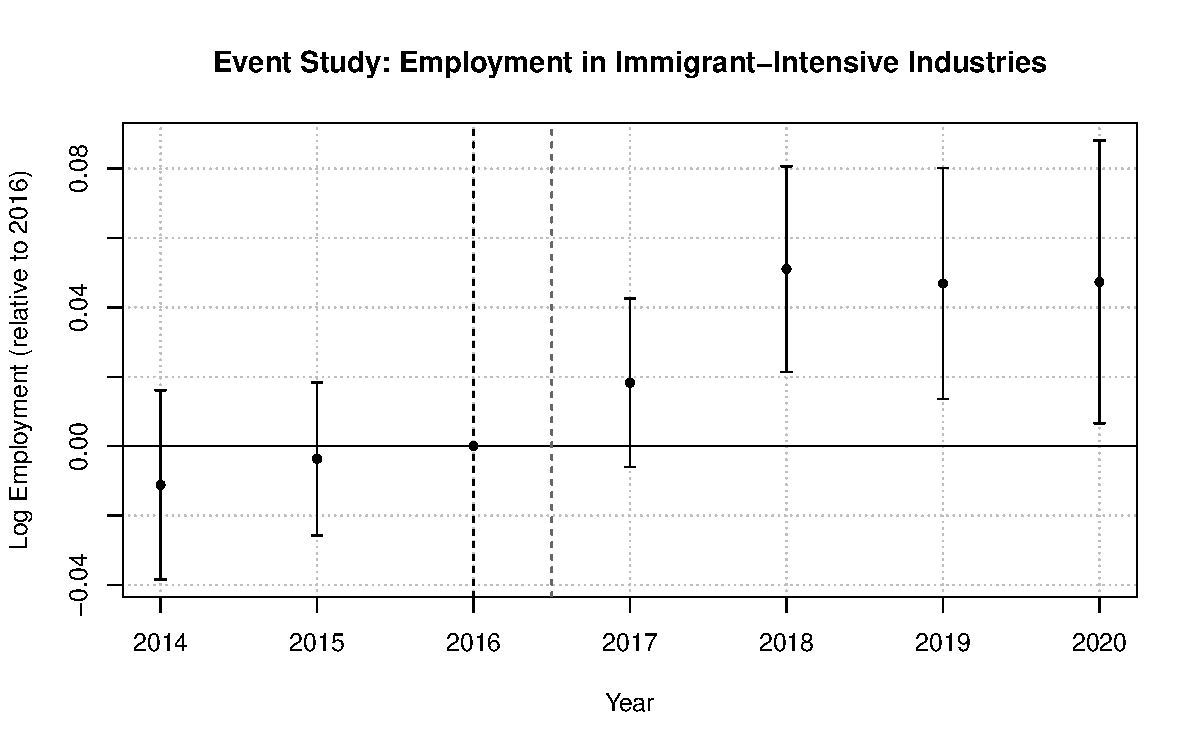
\includegraphics[width=0.85\textwidth]{event_study_plot.pdf}
\caption{Event Study: Employment in Immigrant-Intensive Industries}
\begin{minipage}{0.85\textwidth}
\vspace{6pt}
\small\textit{Notes:} Event study estimates of log employment in target
industries (agriculture, construction, food manufacturing, food services).
High-immigrant states defined as those above the median pre-treatment
immigrant labor share (2014--2016). Coefficients are relative to 2016.
Dashed vertical line marks treatment onset (2017). 95\% confidence
intervals shown. Standard errors clustered at the state level.
\end{minipage}
\end{figure}


\end{document}
 